\section{Performance Analysis}
\label{sec:performance}

We evaluate the performance impact of \system{} in comparison to a CDN that does not perform extra cryptographic operations by simulating both systems.   
We use a series of Virtual Private Servers (VPSs), where each VPS represents a stakeholder in \system{}; Figure \ref{fig:perf_setup} shows our 
experimental setup.  The design of \system{} will likely affect the time that it takes a content publisher to publish her data as
the data has to obfuscated.  Therefore, we measure the time it takes to obfuscate data.  Additionally, \system{} may affect the performance of web page retrieval; therefore, we measure the time to retrieve a objects of varying sizes.  Additionally, we simulate and analyze cache hit rates with varying numbers of 
shared keys $k$, as a higher number of shared keys will result in a lower cache hit rate, and thus negatively affect performance. Analyzing the relationship between cache hit
rates and the number of shared keys can help determine the optimal number of shared keys that should be used in \system{}.

When implementing \system{}, we used SHA-256 for the HMAC implementation and AES-128 for symmetric key cryptographic operations.  We used the {\tt cryptography} library and implemented 
all cryptographic operations in Python.  

\begin{figure}[t]
\centering
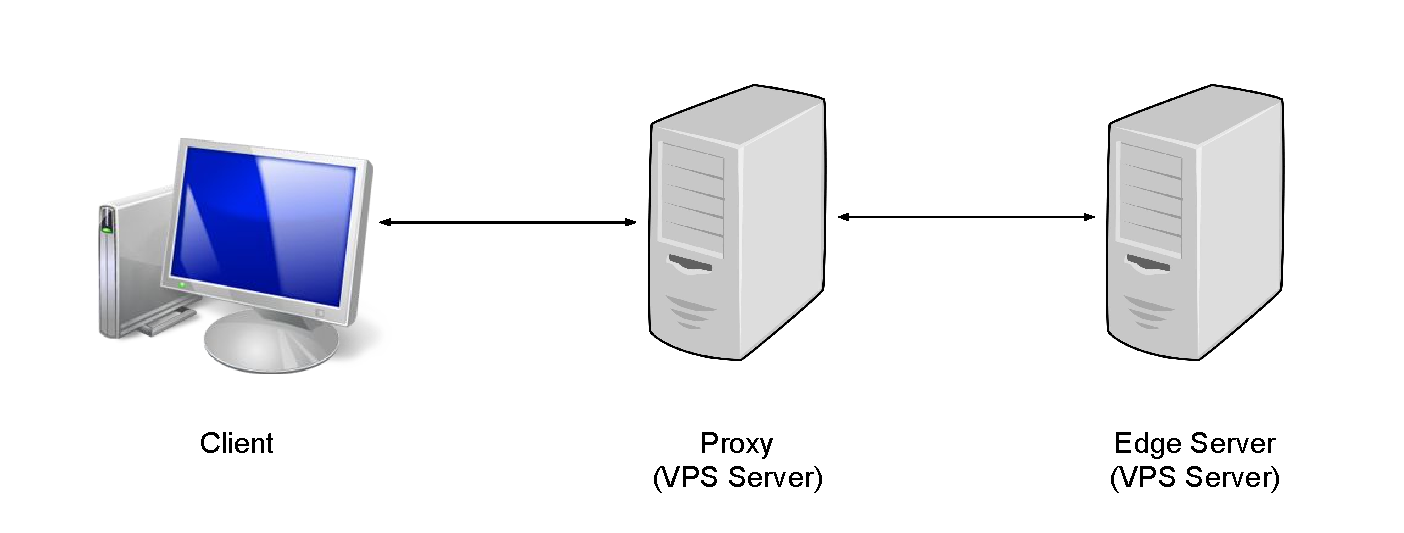
\includegraphics[width=.5\textwidth]{perf_setup}
\caption{Our experimental setup used to evaluate the performance overhead of \system{}.}
\label{fig:perf_setup}
\end{figure}

\subsection{Obfuscation Overhead: Publishing}
As content publishers must compute the HMAC$_k$(URL) and \{content\}$_k$, the act of publishing potentially 
takes longer than not having to perform any cryptographic operations.  In this experiment, we analyze the overhead 
the publisher faces when obfuscating her content.\\

{\bf Metrics}
When comparing the time to publish using \system{} to a typical CDN, the only difference is the obfuscation of 
data (as discussed in Section \ref{sec:publish_protocol}).  This results in our analysis simply of the 
obfuscation; the metric of interest is the total time it takes to encrypt content.  \\

{\bf Experimental Setup}
In our experiment, we setup a client, a proxy, and an edge server. For this experiment, the only machine necessary is 
the edge server --- we are not concerned with the amount of time it takes for the content to be transmitted from 
the publisher's origin server to the edge server, only the amount of time the content publisher takes to obfuscate the data.  Therefore, 
the content and URL are obfuscated on the edge server, and the time it takes to do these operations is measured.  This 
measurement is taken for obfuscating the following file sizes: .000001MB, .001MB, .01MB, .1MB, 1.0MB, 10.0MB, and 100.0MB. \\

{\bf Results}
The results of time to obfuscate data are shown in Figure \ref{fig:encrypt_time}.  We can see that the overhead 
is relatively small for file sizes less than 100.0MB.  In addition, this publishing overhead has no performance impact 
on a client's experience of retrieving, as the client never has to encrypt the content.  

\begin{figure}[t]
\centering
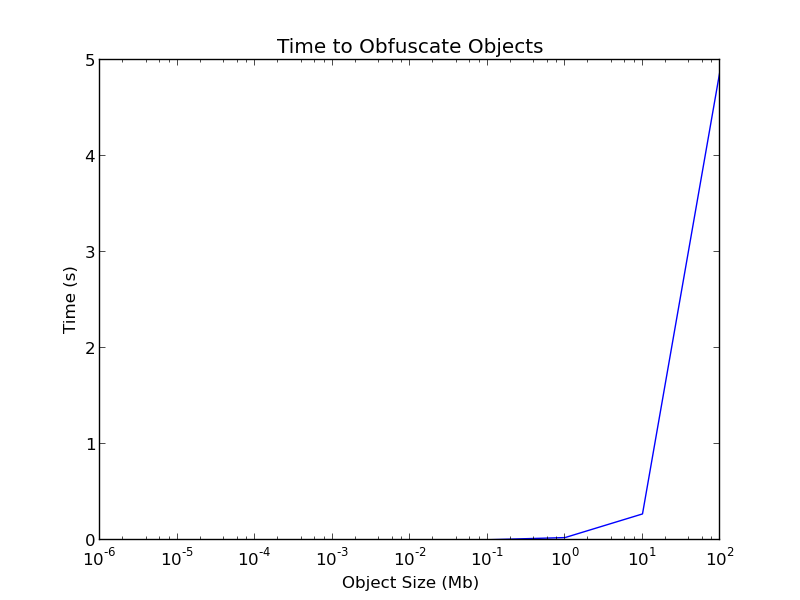
\includegraphics[width=.5\textwidth]{encrypt_time3}
\caption{The time it takes to encrypt/obfuscate different sizes of objects in \system{}.}
\label{fig:encrypt_time}
\end{figure}

\subsection{Obfuscation Overhead: Retrieving}
There is also some overhead associated with retrieving objects when using \system{} due to the operations that 
the proxy must perform.  \\

{\bf Metrics}
We are interested in measuring the affect of cryptographic functions on the retrieval of single 
objects.  The metric used to do so is the end-to-end time to download a single object.  \\

{\bf Experimental Setup}
In our experiment, we setup a client, a proxy, and an edge server.  The client is a  Fujitsu CX2570 M2 servers with dual, 
14-core 2.4GHz Intel Xeon E5 2680 v4 processors with 384GB RAM running the Springdale distribution of Linux machine, 
and both the proxy and edge servers are VPSs running Ubuntu 12.04 x64 LTS with 10GB of storage. The proxy is located in 
Montreal, Canada, and the edge server is located in Chicago, USA.  To account for any additional latency on the links between 
the client and proxy, or proxy and edge server, we treat a traditional CDN as a system of client, proxy, and edge server, where 
the edge server acts as a simple proxy and does not perform any operations.  

First, different sizes of objects are generated, encrypted, and obfuscated on the edge server; the sizes of objects we create are: 
.000001MB, .001MB, .01MB, .1MB, 1.0MB, 10.0MB, and 100.0MB.  These are the objects that will be downloaded by the client, and we 
assume all objects are in the cache, as the time it takes the CDN to fetch the content from the origin server (if there is a cache 
miss) should not differ between \system{} and a traditional CDN. 

Our proxy runs {\tt mitmproxy}, which allows for interception and manipulation of HTTP requests and responses.  We implement 
these modifications at the proxy.  

In this experiment, the client machine requests the objects using {\tt curl} with specific options to use the designated proxy, 
and to measure the transfer time.  \\

\begin{figure}[t]
\centering
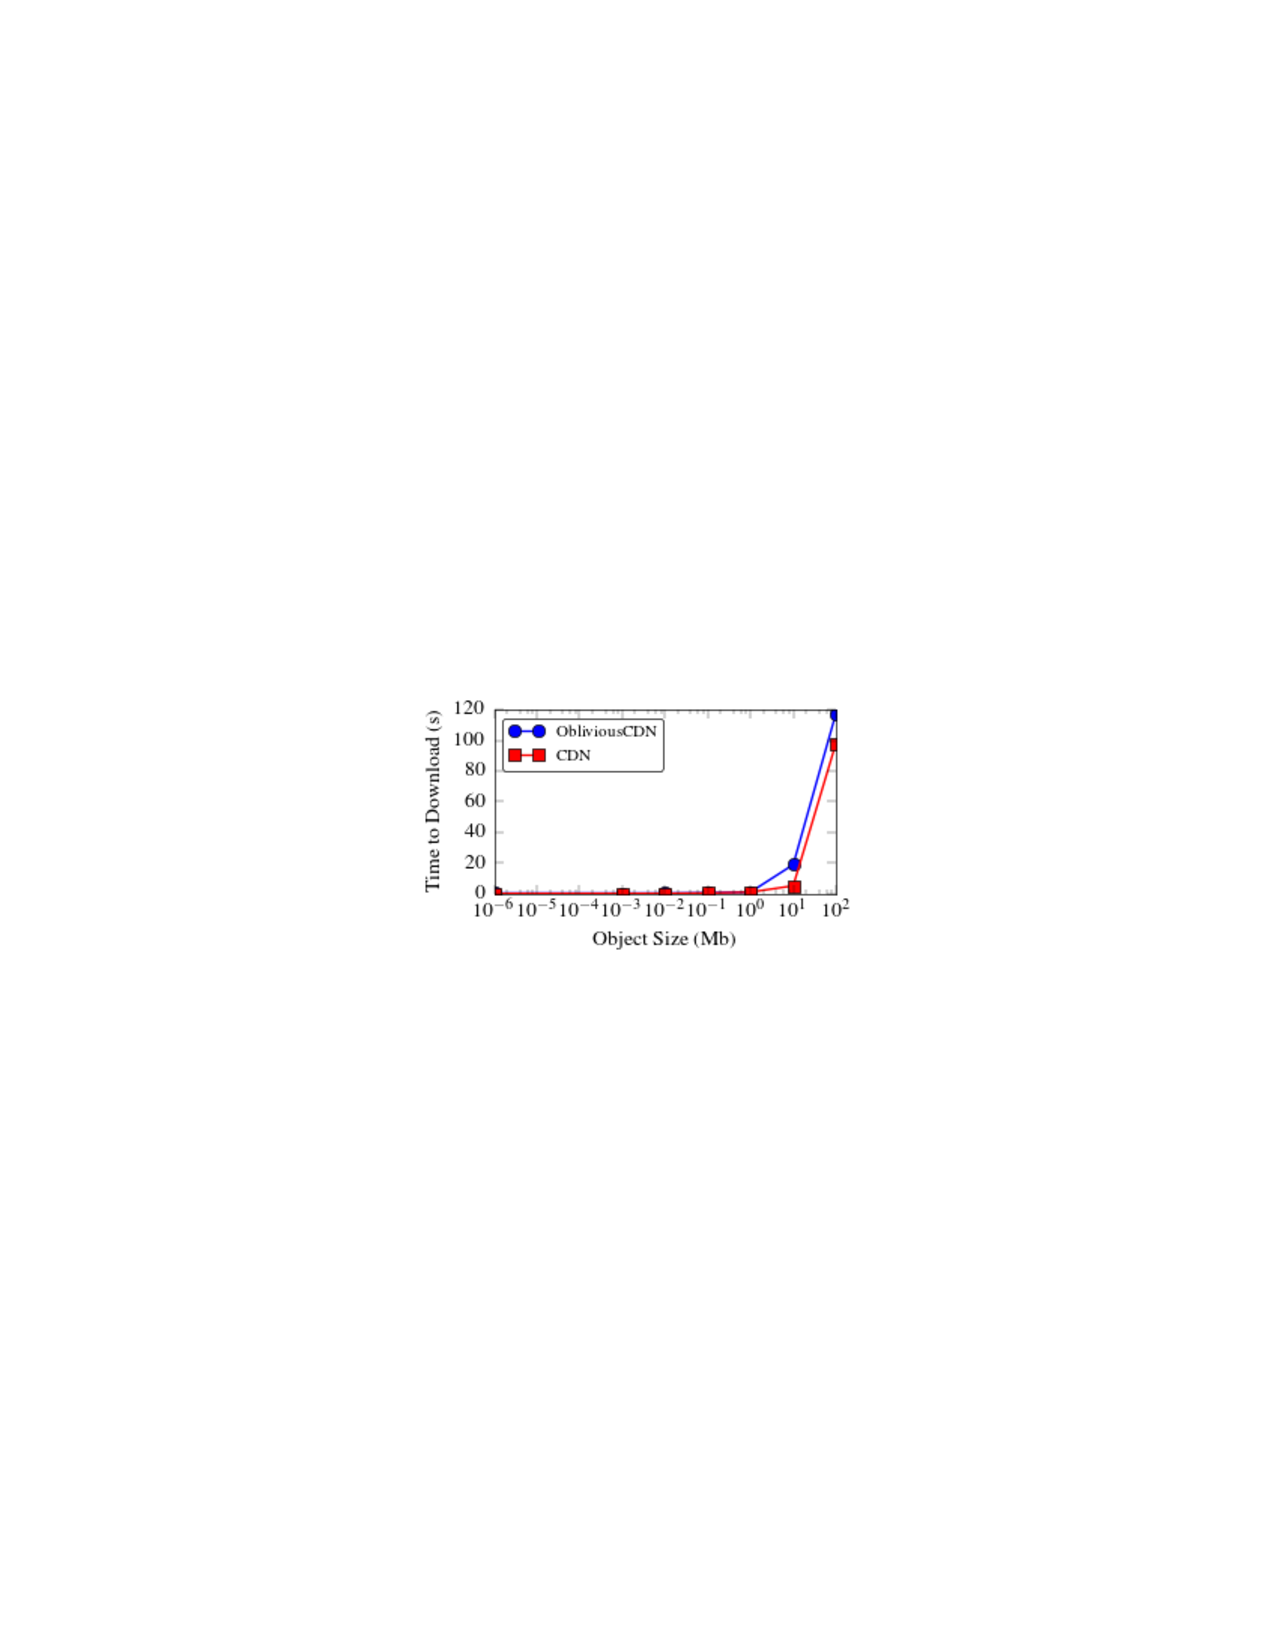
\includegraphics[width=.5\textwidth]{transfer}
\caption{The total transfer time for accessing different sizes of objects using \system{} and without \system{}'s cryptographic operations.}
\label{fig:transfer}
\end{figure}

{\bf Results}
After conducting the experiment, we find the results shown in Figure \ref{fig:transfer}.  We can see that total download times are comparable 
for objects that are smaller than 10MB; objects larger than 10MB take slightly longer to download using \system{} than a traditional CDN, 
due to the cryptographic operations performed at the proxy.  

Additionally, recent work has reported that the average object size retrieval from Akamai is only 335 Kb, and the average object size 
of popular objects ($>$ 200,000 requests) is only 8.6 Kb~\cite{berger2016achieving}.  Both of these object sizes are less than 10MB, resulting in negligible 
performance differences between \system{} and a traditional CDN.

\subsection{Cache Hit Rates}
The other reason for lower performance in \system{} is because there are fewer copies of the content that a single proxy can request.  As each set 
of proxies use a different shared key, and these proxies can only request the content encrypted with their shared key, this can lead to high cache misses.  
This would cause the CDN to fetch the object from the content publisher's server, which increases the latency, and degrades performance for the client.  
In this experiment, we measure just how much of an impact the number of shared keys has on the cache hit rate.\\

{\bf Metrics}
In addition to the use of proxies and cryptographic operations, \system{} could suffer performance losses from lower cache hit ratios.  As the number 
of shared keys (between the proxies and the content publishers' servers) increases, the cache hit ratio will likely decrease.  The metric we are interested 
in to evaluate the performance impact of multiple shared keys is the cache hit ratio.\\

{\bf Experimental Setup}
In this experiment, we simulate the cache hit rate with a fixed number of clients while varying the number of shared keys $k$.  We use 
access logs from prior research~\cite{andersen2005improving} to simulate cache requests, and we assume a cache size of 1.2 GB~\cite{berger2017adaptsize} and that all objects have 
the same size of 12 KB~\cite{berger2016achieving}.  The experiment starts with a cold cache, five clients, and a single shared key; this is 
replicated five times, where we increase the number of shared keys by one each time, resulting in an analysis of how the cache hit rate is affected 
by values of $1~<=~k~<= 5$.

{\bf Results}
